\documentclass{beamer}

\usepackage[english]{ babel }
\usepackage[T1]{ fontenc }
\usepackage{ graphicx }
\graphicspath{ {./pix/} }

\usetheme[block=fill]{m}

\title{Shikata ga nai}
\author{Radare2 workshop}
\date{\today}
\institute{hack.lu 2015}

\begin{document}

\maketitle

\begin{frame}{Disclaimer}
	\begin{center}
		This workshop is based on ideas and scripts from\\
		Jaime (\alert{@NighetMan}) Peñalba.
	\end{center}
\end{frame}

\begin{frame}{Where to find the material?}
	\begin{center}
		Please look at the \alert{shikata\_ga\_nai} folder in the virtual machine
	\end{center}
\end{frame}

\section{What are we going to do?}

\begin{frame}{Shikata ga nai}
	\begin{center}
		Unpack \alert{Shikata ga nai}!
	\end{center}
	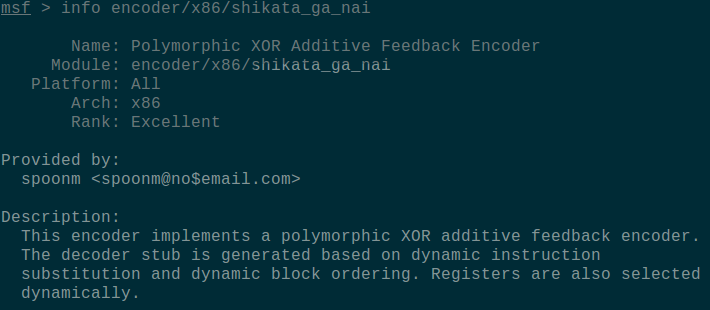
\includegraphics[width=\textwidth]{description.png}
\end{frame}

\begin{frame}{Shikata ga nai}
	\begin{itemize}
		\item Polymorphic
		\item 320 lines of msf-powered OOP Ruby
		\item We want the unpacked shellcode
	\end{itemize}
\end{frame}

\section{How do we do it?}

\begin{frame}{Solutions}
	\begin{itemize}[<+->]
		\item Run it on your machine and see what happens
		\item Step-step-step-step-step-… in gdb
		\item Trace the execution in a virtual machine
		\item Use radare2 with \alert{ESIL}!
	\end{itemize}
\end{frame}

\section{But what is ESIL?}

\begin{frame}{ESIL}
	\begin{itemize}
		\item Evaluable String Intermediary Language
		\item Yet another intermediary language
		\item RPN-ish
		\item \alert{$jz\;0xaabbccdd$} :  $zf,?{,0xaabbccdd,eip,=,}$
	\end{itemize}
\end{frame}

\section{What can we do with this \emph{ESIL}?}

\begin{frame}{ESIL}
	\begin{columns}
		\begin{column}{.4\textwidth}
			\begin{itemize}
				\item Used for
					\begin{itemize}[<+->]
						\item Emulation
						\item Decompilation
						\item Analysis
						\item Flamewars against other IL
					\end{itemize}
			\end{itemize}
		\end{column}
		\begin{column}{.6\textwidth}
			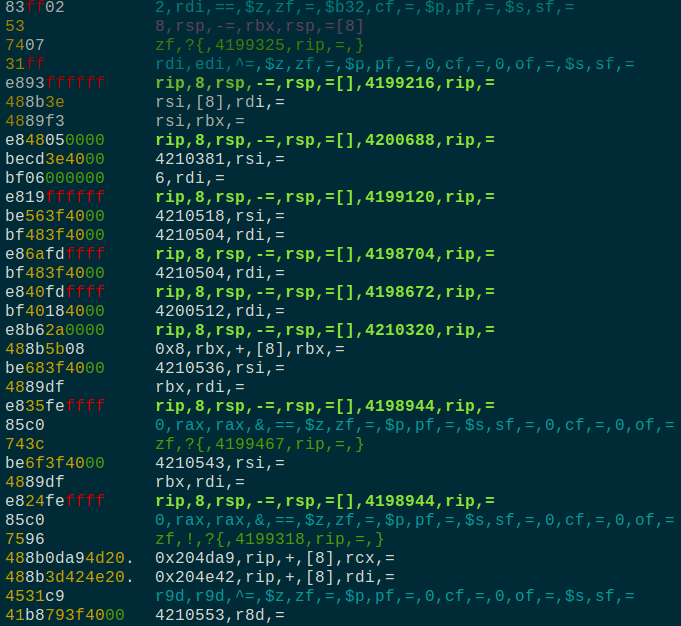
\includegraphics[width=\textwidth]{esil.png}
		\end{column}
	\end{columns}
\end{frame}

\section{How does emulation help us to dump the shellcode?}

\begin{frame}{Where to stop?}
	We can emulate the shellcode, but \alert{where} do we stop?
	\begin{itemize}
		\item Instructions aren't fixed.
		\item Blocks are permutated.
		\item Registers are dynamically selected.
	\end{itemize}
	\begin{center}
		So what can we do?
	\end{center}
\end{frame}

\begin{frame}{Reading the source code}
	It seems that the last instruction will always be \alert{loop}.
	\newline
	\newline
	\pause
	So we can emulate the shellcode, and dump the result from the last \alert{loop} instruction
	till then end.
\end{frame}

\section{How do we use radare2/ESIL anyway?}

\begin{frame}{r2pipe}
	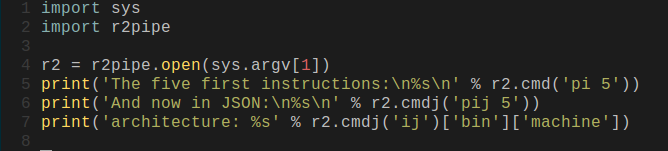
\includegraphics[width=\textwidth]{r2pipe.png}
\end{frame}

\begin{frame}{Languages}
	\begin{block}{NodeJS}
		npm install r2pipe
	\end{block}
	\begin{block}{Python}
		pip install r2pipe
	\end{block}
	\begin{block}{Ruby}
		gem install r2pipe
	\end{block}
\end{frame}

\section{So let's use ESIL?}

\begin{frame}{Plot twist}
	\only<1>{
		\begin{itemize}
			\item FPU is currently not supported in ESIL :D
			\item FPU is used to get EIP with \alert{FNSTENV}
			\item Polymorphic FPU instructions
		\end{itemize}
	}
	\only<2>{
		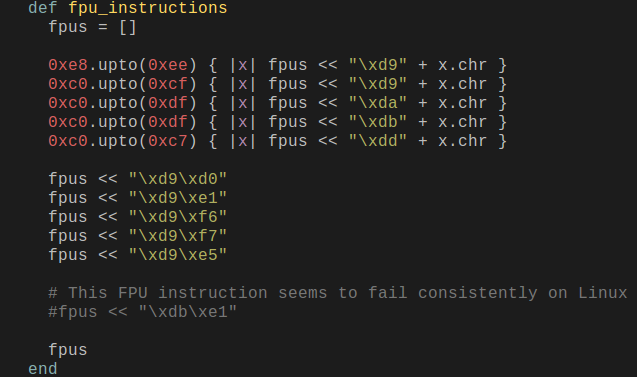
\includegraphics[width=\textwidth]{fpu.png}
	}
\end{frame}

\section{Can we emulate them the \emph{ghetto way}?}

\begin{frame}{Are those detected as FPU by r2?}
	\begin{itemize}
		\item You've got the \alert{hello\_world.py} code
		\item Check if every opcode in the \alert{test\_fpu.py} one has the \alert{fpu} family
		\item Feel free to do it in your favourite language!
	\end{itemize}
\end{frame}

\begin{frame}{My solution}
	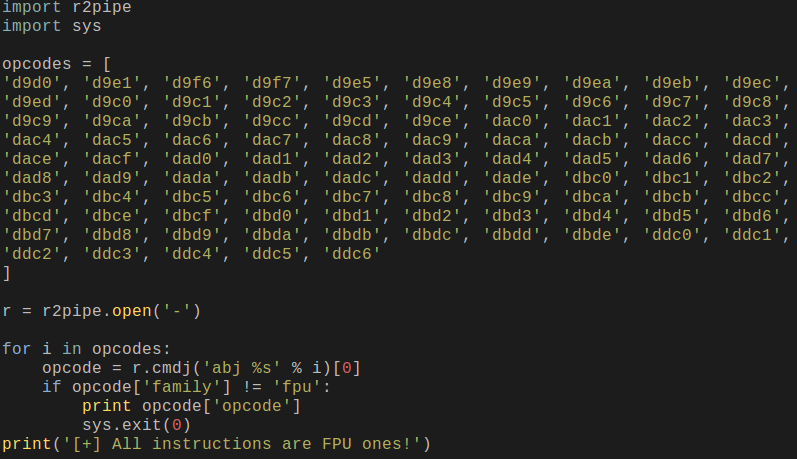
\includegraphics[width=\textwidth]{fpus.png}
\end{frame}

\section{Ready to unpack shikata ga nai?}

\begin{frame}{Sum up}
	\begin{enumerate}
		\item Initialize the ESIL vm
		\item If the instruction is \alert{invalid}
			\begin{enumerate}
				\item We're at the end!
				\item Dump from the last encountered \alert{loop} instruction to the end
			\end{enumerate}
		\item Else, if the instruction is an fpu one
			\begin{enumerate}
				\item If it's \alert{fnstenv}, write the previously stored \alert{eip} at \alert{esp}
				\item Else, store \alert{eip}
			\end{enumerate}
		\item Else, if the instruction is \alert{loop}, store its location
		\item Step and goto \emph{2}.
	\end{enumerate}
\end{frame}

\section{Your turn!}

\begin{frame}{My solution}
	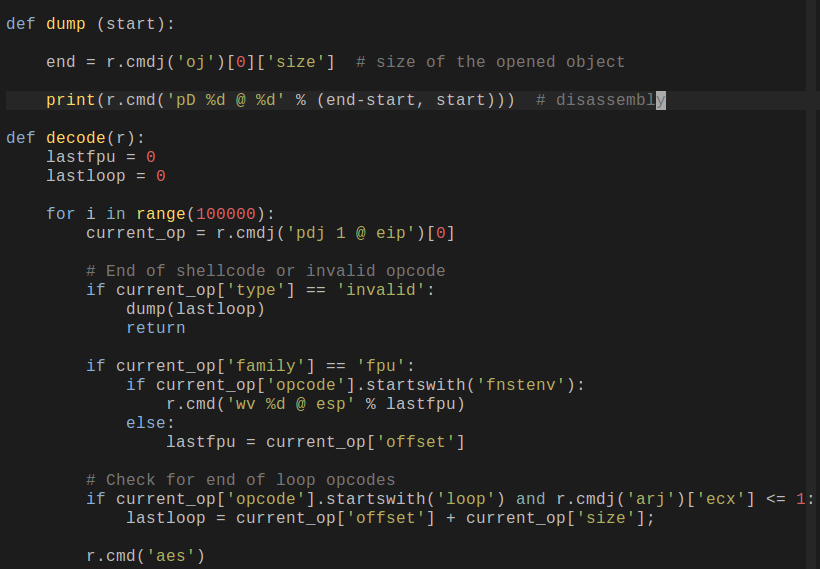
\includegraphics[width=\textwidth]{solution.png}
\end{frame}

\section*{Conclusion}
\begin{frame}{Conclusion}
	\begin{center}
	\only<1>{
		\begin{itemize}
			\item ESIL is cool
			\item Still WIP
			\item More to come!
		\end{itemize}
	}
	\only<2>{
		\Large
		Radare2 is \alert{nice}.

		You should use it.
	}
	\end{center}
\end{frame}

\begin{frame}{Resources}
	\begin{itemize}
		\item \href{https://github.com/radare/radare2}{Github repo}
		\item \href{http://rada.re}{Official website}
		\item \href{http://radare.today}{The r2 blog}
		\item \href{http://maijin.github.io/radare2book/}{The r2 book}
		\item \href{https://twitter.com/radareorg}{Twitter}
	\end{itemize}
\end{frame}

\end{document}
